\documentclass[11pt,twoside,a4paper]{article}
% http://www-h.eng.cam.ac.uk/help/tpl/textprocessing/latex_maths+pix/node6.html symboles de math
% http://fr.wikibooks.org/wiki/Programmation_LaTeX Programmation latex (wikibook)
%=========================== En-Tete =================================
%--- Insertion de paquetages (optionnel) ---
\usepackage[french]{babel}   % pour dire que le texte est en fran{\'e}ais
\usepackage{a4}				 % pour la taille   
\usepackage[T1]{fontenc}	 % pour les font postscript
\usepackage{epsfig}		  % pour gerer les images
%\usepackage{psfig}
\usepackage{amsmath, amsthm} % tres bon mode mathematique
\usepackage{amsfonts,amssymb}% permet la definition des ensembles
\usepackage{float}		   % pour le placement des figure
\usepackage{verbatim}

\usepackage{longtable} % pour les tableaux de plusieurs pages

\usepackage[table]{xcolor} % couleur de fond des cellules de tableaux

\usepackage{lastpage}

\usepackage{multirow}

\usepackage{multicol} % pour {\'e}crire dans certaines zones en colonnes : \begin{multicols}{nb colonnes}...\end{multicols} 

% \usepackage[top=1.5cm, bottom=1.5cm, left=1.5cm, right=1.5cm]{geometry}
% gauche, haut, droite, bas, entete, ente2txt, pied, txt2pied
\usepackage{vmargin}
\setmarginsrb{1.0cm}{1.0cm}{1.0cm}{1.0cm}{15pt}{3pt}{100pt}{30pt}

\usepackage{lscape} % changement orientation page
%\usepackage{frbib} % enlever pour obtenir references en anglais
% --- style de page (pour les en-tete) ---
\pagestyle{headings}

% % % en-tete et pieds de page configurables : fancyhdr.sty

% http://www.trustonme.net/didactels/250.html

% http://ww3.ac-poitiers.fr/math/tex/pratique/entete/entete.htm
% http://www.ctan.org/tex-archive/macros/latex/contrib/fancyhdr/fancyhdr.pdf
\usepackage{fancyhdr}
\pagestyle{fancy}
% \newcommand{\chaptermark}[1]{\markboth{#1}{}}
% \newcommand{\sectionmark}[1]{\markright{\thesection\ #1}}
\fancyhf{}
\fancyhead[LE,RO]{\bfseries\thepage}
\fancyhead[LO]{\bfseries\rightmark}
\fancyhead[RE]{\bfseries\leftmark}
\fancyfoot[LE]{\thepage /\pageref{LastPage} \hfill
	OAuth2 -- \emph{Confidentiel *****}
\hfill 
\includegraphics[width=0.5cm]{img/logo_glider.png} }
\fancyfoot[RO]{
\includegraphics[width=0.5cm]{img/logo_glider.png} \hfill
	\emph{Confidentiel *****} -- OAuth2
\hfill \thepage /\pageref{LastPage}}
\renewcommand{\headrulewidth}{0.5pt}
\renewcommand{\footrulewidth}{0.5pt}
\addtolength{\headheight}{0.5pt}
\fancypagestyle{plain}{
	\fancyhead{}
	\renewcommand{\headrulewidth}{0pt}
}

\renewcommand{\headrulewidth}{0.25pt}
\renewcommand{\footrulewidth}{0.5pt}
%% \setlength{\headheight}{85pt}
% \addtolength{\headheight}{0.5pt}
% \fancypagestyle{plain}{
% 	\fancyhead{}
% 	\fancyfoot{}
% 	\renewcommand{\headrulewidth}{0pt}
% }

%--- Definitions de nouvelles commandes ---
\newcommand{\N}{\mathbb{N}} % les entiers naturels


%--- Pour le titre ---
\def\maketitle{%
	\begin{center}
		\begin{tabular}[c]{c|c}
			\textsc{\textbf{Institution}}~\\[\baselineskip]~\\[\baselineskip]
			\emph{\textbf{Date 09-09-2009}}~\\[\baselineskip]~\\[\baselineskip]
			\emph{\textbf{Pr{\'e}cisions relatives au contexte}}~\\[\baselineskip]~\\[\baselineskip]
			\textsc{Auteur inestimable}~\\[\baselineskip]~\\[\baselineskip]
			& 
			
\includegraphics[width=3cm]{img/logo_glider.png}~\\[\baselineskip]
		\end{tabular}
		% \\ \hline
		 	% % if more than one logo
			% 
\includegraphics[width=5cm]{img/logo_glider.png}
			% \includegraphics[width=5cm]{img/logo_wifi.png}
		% \\ \hline
		% \end{tabular}
			~\\[\baselineskip]~\\[\baselineskip]
			\Huge{Titre principal}~\\[\baselineskip]
			\Large{Titre secondaire}~\\[\baselineskip]
		
		~\\[\baselineskip]
		~\\[\baselineskip]
	\large{
		\textsc{\textbf{Institution d'accueil et jury}}
		~\\[\baselineskip]
		<<titre personne>> : \texttt{Anne ONYME}~\\[\baselineskip]
		<<titre personne>> : \texttt{Jocelyn CONNU}~\\[\baselineskip]
		~\\[\baselineskip]
		\textit{Pr{\'e}cisions du contexte de r{\'e}daction de l'article}
	}

	\end{center}

}%



%--- Pour le glossaire --- a defaut de \makeglossary ou d'utilisation d'index latex

\definecolor{verylightgray}{rgb}{0.8,0.8,0.8}
\def\makeglossaire{%
	\begin{center}

	\begin{tabular}{|>{\columncolor{verylightgray}} p{0.2\textwidth}|p{0.8\textwidth}|}

		\hline

		\textbf{BLAST} & 

			\begin{tabular}{p{0.8\textwidth}}

			Basic Local Alignment Search Tool \\

			\textit{algorithmes et logiciels pour l'alignement de s{\'e}quences et la recherche de similarit{\'e}s locales}

			\end{tabular} \\

		\hline

		\textbf{BNDB} & Biochemical NetWork DataBase \textit{(entrep{\^o}t de donn{\'e}es)} \\

		\hline

	\end{tabular}

\end{center}

}%

%============================= Corps =================================
\begin{document}

%% %ecrire le titre...
%% \maketitle
%% \setcounter{page}{0}
%% \thispagestyle{empty}
%% \clearpage
%% \setcounter{page}{0}
%% \thispagestyle{empty}
%% ~\\
%% \clearpage
%% \setcounter{page}{0}
%% \thispagestyle{empty}
%% % ecrire la table des mati{\'e}res...
%% \tableofcontents
%% % \clearpage
%% % \setcounter{page}{0}
%% % \thispagestyle{empty}
%% % ecrire la table des figures et celle des tableaux
%% \setcounter{page}{0}
%% \thispagestyle{empty}
%% ~\\ \rule{10cm}{1mm}~\\
%% \listoffigures
%% ~\\ \rule{10cm}{1mm}~\\
%% \listoftables
%% \clearpage

\setlength\parindent{0pt}

\setcounter{page}{1}

\texttt{http://blog.netapsys.fr/oauth-comment-ca-marche/comment-page-1/}

\textbf{\Large OAuth : Comment \c{c}a marche ?}~\\

\emph{26 d{\'e}cembre 2014 --- Hoby RATSITOBAINA}~\\

Vous avez s{\^u}rement remarqu{\'e} que certains sites nous proposent de nous authentifier {\`a} partir de nos comptes Facebook ou Twitter ou encore Google + et ainsi r{\'e}cup{\'e}rer les informations de notre  profil. En tant qu'utilisateur cela est bien pratique, mais savez-vous ce qui se passe dans les coulisses ? ~\\

Cette fonctionnalit{\'e} est rendue possible gr{\^a}ce {\`a} une API s{\'e}curis{\'e}e propos{\'e}e par Facebook, Twitter, Google+. Ces derniers proposent {\'e}galement plusieurs API permettant de faire un peu de tout avec votre compte. En ayant connaissance de cette information, il est donc possible que le site sur lequel vous vous connectez puisse tout faire avec votre compte. Avez-vous int{\'e}r{\^e}t {\`a} vous y connecter, {\`a} lui fournir vos identifiants de connexion ? ~\\

Pour pallier ces craintes, la solution est de mettre en place un m{\'e}canisme de d{\'e}l{\'e}gation d'autorisation entre les diff{\'e}rentes entit{\'e}s. OAuth a {\'e}t{\'e} cr{\'e}e dans ce sens. ~\\

\section*{Qu'est-ce que OAuth ?\markboth{Qu'est-ce que OAuth ?}{Qu'est-ce que OAuth ?}}
\addcontentsline{toc}{section}{Qu'est-ce que OAuth ?}

\begin{minipage}[t]{0.20\textwidth}
	% \begin{figure}[ht]
		
\includegraphics[width=0.95\textwidth]{img/oauth-2-sm.png}
		% \caption{figure}{OAuth 2.0}
	% \end{figure}
\end{minipage} \hfill \begin{minipage}[h]{0.80\textwidth}
	OAuth est un protocole libre qui permet d'autoriser une application client {\`a} utiliser l'API s{\'e}curis{\'e}e d'une autre application pour le compte d'un utilisateur. ~\\

	L'int{\'e}r{\^e}t majeur d'OAuth vient du fait que l'utilisateur n'a plus besoin de fournir ses informations d'identification {\`a} une application tierce car la connexion se passe sur l'application de l'API. Cela suppose que l'utilisateur lui a {\`a} priori fait confiance. ~\\

	Actuellement, OAuth est {\`a} la version 2.0. Voyons ensembles les notions de base de l'OAuth. ~\\
\end{minipage}

\subsection*{Les r{\^o}les\markboth{Les r{\^o}les}{Les r{\^o}les}}
\addcontentsline{toc}{subsection}{Les r{\^o}les}

OAuth propose 4 r{\^o}les :
\begin{itemize}
	\item[$>$] \textbf{Ressource Owner (Le d{\'e}tenteur des donn{\'e}es)}~\\
	Il s'agit d'une entit{\'e} capable d'accorder l'acc{\`e}s {\`a} une ressource prot{\'e}g{\'e}e. Lorsque le propri{\'e}taire de la ressource est une personne, il est d{\'e}sign{\'e} en tant qu'utilisateur final.
	\item[$>$] \textbf{Ressource Server (Le serveur de ressources)}~\\
	Il s'agit d'un serveur qui h{\'e}berge les ressources prot{\'e}g{\'e}es, qui est capable d'accepter et de r{\'e}pondre aux demandes de ressources prot{\'e}g{\'e}es en utilisant des jetons d'acc{\`e}s (Access Token).
	\item[$>$] \textbf{Client (Le client)}~\\
	Il s'agit d'une application demandant des ressources prot{\'e}g{\'e}es au nom du propri{\'e}taire de celles-ci et avec son autorisation. Cela peut-{\^e}tre une application PHP c{\^o}t{\'e} serveur,  une application JavaScript c{\^o}t{\'e} client, une application mobile.
	\item[$>$] \textbf{Authorization Server (Le serveur d'autorisation)}~\\
	Il s'agit d'un serveur qui d{\'e}livre des jetons d'acc{\`e}s (Access Token) au client apr{\`e}s que le propri{\'e}taire de la ressource a {\'e}t{\'e} formellement authentifi{\'e} et qu'il a obtenu une autorisation de sa part.
\end{itemize} ~\\

Ci-dessous un r{\'e}sum{\'e} des flux du protocole OAuth :

\begin{figure}[ht]
	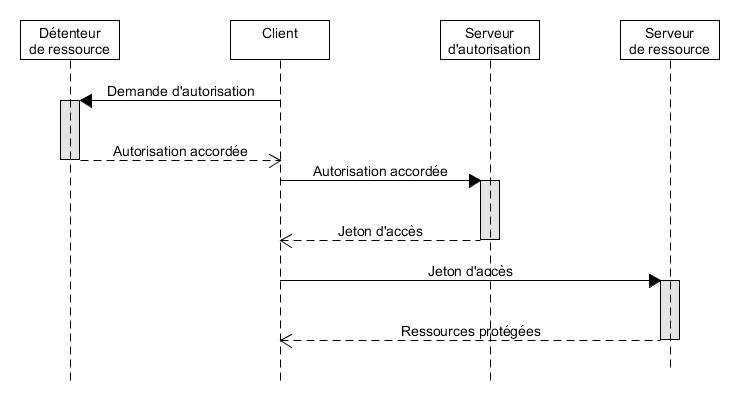
\includegraphics[width=0.85\textwidth]{img/Resume_flux_OAuth.jpg}
	\caption{R{\'e}sum{\'e} des flux du protocole OAuth 2.0}
\end{figure}

\subsection*{Le token\markboth{Le token}{Le token}}
\addcontentsline{toc}{subsection}{Le token}

Le token est une cha{\^i}ne de caract{\`e}res, il est {\'e}mit par le serveur d'autorisation {\`a} la demande du client. Le serveur d'autorisation d{\'e}finit sa dur{\'e}e de vie et les valeurs des autres param{\`e}tres.

\begin{itemize}
	\item[$>$] Access token (jeton d'acc{\`e}s)~\\
	Le jeton d'acc{\`e}s permet au client d'acc{\'e}der aux ressources prot{\'e}g{\'e}es d'un utilisateur sur le serveur de ressources. A chacune des requ{\^e}tes du client vers le serveur de ressources, le token est envoy{\'e} soit en param{\`e}tre soit dans un header de la requ{\^e}te. Il doit rester confidentiel d{\`e}s que possible.
	\item[$>$] Refresh token (jeton de renouvellement)~\\
	Le jeton de renouvellement est un token pour renouveler le jeton d'acc{\`e}s lorsque ce dernier est expir{\'e}. Le client envoie le jeton de renouvellement au serveur d'autorisation pour obtenir un nouveau jeton d'acc{\`e}s. Le jeton de renouvellement est d{\'e}livr{\'e} en m{\^e}me temps que le jeton d'acc{\`e}s, cependant il n'est pas envoy{\'e} {\`a} chaque requ{\^e}te du client.
\end{itemize}

\subsection*{Les scopes\markboth{Les scopes}{Les scopes}}
\addcontentsline{toc}{subsection}{Les scopes}

Le scope est un param{\`e}tre qui d{\'e}finit la port{\'e}e des droits de la demande d'autorisation. La liste des scopes est d{\'e}finie au niveau du serveur d'autorisation. --- Le client doit pr{\'e}ciser le ou les scopes qu'il souhaite utiliser lors de la demande d'autorisation.

\subsection*{HTTPS\markboth{HTTPS}{HTTPS}}
\addcontentsline{toc}{subsection}{HTTPS}

OAuth impose l'utilisation de HTTPS pour les {\'e}changes entre le client et le serveur d'autorisation du fait des donn{\'e}es sensibles qui transitent entre les deux (jeton d'acc{\`e}s, {\'e}ventuellement des identifiants et des mots de passe). --- HTTP est un protocole de communication client-serveur d{\'e}velopp{\'e} pour le World Wide Web. --- HTTPS n'est autre que la combinaison du HTTP avec une couche de chiffrement comme SSL ou TLS. 

\section*{Les types de Client\markboth{Les types de Client}{Les types de Client}}
\addcontentsline{toc}{section}{Les types de Client}

OAuth a d{\'e}fini deux types de client, bas{\'e}s sur leur capacit{\'e} {\`a} s'authentifier en toute s{\'e}curit{\'e} sur le serveur d'autorisation.

\subsection*{Confidentiel (Confidential)\markboth{Confidentiel (Confidential)}{Confidentiel (Confidential)}}
\addcontentsline{toc}{subsection}{Confidentiel (Confidential)}

Il s'agit d'un client qui a la capacit{\'e} de maintenir la confidentialit{\'e} de ses informations d'identification ou de s{\'e}curiser l'authentification client {\`a} l'aide d'autres moyens.

\subsection*{Public (Public)\markboth{Public (Public)}{Public (Public)}}
\addcontentsline{toc}{subsection}{Public (Public)}

Il s'agit d'un client qui a les aptitudes inverses d'un client confidentiel.

\section*{Les diff{\'e}rents profils de client\markboth{Les diff{\'e}rents profils de client}{Les diff{\'e}rents profils de client}}
\addcontentsline{toc}{section}{Les diff{\'e}rents profils de client}

OAuth a d{\'e}fini trois profils client :

\subsection*{Application web (Web application)\markboth{Application web (Web application)}{Application web (Web application)}}
\addcontentsline{toc}{subsection}{Application web (Web application)}

Une application Web est un client de type confidentiel qui fonctionne sur un serveur web. --- La ressource prot{\'e}g{\'e}e du propri{\'e}taire est accessible par le client via une interface utilisateur en HTML rendu par un user-agent (par exemple, navigateur Web) d'un dispositif utilis{\'e} par le propri{\'e}taire de la  ressource. ~\\

Les informations d'identification du client ainsi que le jeton d'acc{\`e}s {\'e}mis au client sont stock{\'e}s sur le serveur web et sont non expos{\'e}s ou non accessibles par le propri{\'e}taire de la ressource.

\subsection*{Application bas{\'e}e sur un user-agent (User-agent-based application)\markboth{Application bas{\'e}e sur un user-agent (User-agent-based application)}{Application bas{\'e}e sur un user-agent (User-agent-based application)}}
\addcontentsline{toc}{subsection}{Application bas{\'e}e sur un user-agent (User-agent-based application)}

Une application bas{\'e}e sur un user-agent est un client de type public dans lequel le code client est t{\'e}l{\'e}charg{\'e} {\`a} partir d'un serveur Web et ex{\'e}cut{\'e} sur un user-agent (par exemple, navigateur Web) d'un dispositif utilis{\'e} par le propri{\'e}taire de la  ressource. ~\\

Les donn{\'e}es du protocole et les informations d'identification sont facilement accessibles (et souvent visibles) pour le propri{\'e}taire de la ressource.

\subsection*{Application native (Native application)\markboth{Application native (Native application)}{Application native (Native application)}}
\addcontentsline{toc}{subsection}{Application native (Native application)}

Une application native est un client de type public install{\'e} et ex{\'e}cut{\'e} sur un dispositif utilis{\'e} par propri{\'e}taire de la ressource. ~\\

Les donn{\'e}es du protocole et les informations d'identification sont facilement accessibles (et souvent visible) au propri{\'e}taire de la ressource. Cela suppose que les informations d'identification inclues dans l'application peuvent {\^e}tre extraites.

\section*{Enregistrement du client\markboth{Enregistrement du client}{Enregistrement du client}}
\addcontentsline{toc}{section}{Enregistrement du client}

Avant d'utiliser le protocole OAuth, il faut que le client s'enregistre aupr{\`e}s du serveur d'autorisation.

Le protocole a d{\'e}fini des param{\`e}tres qui doivent {\^e}tre renseign{\'e}s par le client :
\begin{itemize}
	\item[$>$] Sp{\'e}cifier le type de client
	\item[$>$] Fournir les URL de redirection du client
	\item[$>$] Fournir d'autres informations requises par le serveur d'autorisation
\end{itemize} ~\\

\underline{Exemple :}
\begin{itemize}
	\item[$>$] Application Name: le nom de l'application
	\item[$>$] Redirect URLs: les URLs du client vers lesquelles les redirections (contenant le code d'autorisation et le token d'acc{\`e}s) seront effectu{\'e}es par le serveur d'autorisation
	\item[$>$] Grant Type(s): les types d'autorisation qui seront utilis{\'e}es par le client
	\item[$>$] Javascript Origin (optionnel): le nom de domaine qui sera autoris{\'e} {\`a} effectuer des requ{\^e}tes XMLHttpRequest vers le serveur de ressource
\end{itemize} ~\\

En retour de l'enregistrement du client, le serveur d'autorisation renvoie les param{\`e}tres suivants :
\begin{itemize}
	\item[$>$] Client Id: cha{\^i}ne de caract{\`e}res unique et g{\'e}n{\'e}r{\'e}e al{\'e}atoirement
	\item[$>$] Client Secret: cl{\'e} secr{\`e}te qui doit le rester en toute circonstance
\end{itemize}

\section*{Les types d'autorisation\markboth{Les types d'autorisation}{Les types d'autorisation}}
\addcontentsline{toc}{section}{Les types d'autorisation}

Pour demander un jeton d'acc{\`e}s, le client doit obtenir une autorisation du propri{\'e}taire de la ressource. --- OAuth a d{\'e}fini quatre types d'autorisation : Authorization Code Grant, Implicit Grant, Resource Owner Password Credentials Grant, Client Credentials Grant . 

\subsection*{L'autorisation via un code (Authorization Code Grant)\markboth{L'autorisation via un code (Authorization Code Grant)}{L'autorisation via un code (Authorization Code Grant)}}
\addcontentsline{toc}{subsection}{L'autorisation via un code (Authorization Code Grant)}

L'autorisation via un code est utilis{\'e}e pour obtenir en m{\^e}me temps un jeton d'acc{\`e}s et un jeton de renouvellement ce qui permet d'obtenir un jeton d'acc{\`e}s de longue dur{\'e}e. Il est optimis{\'e} pour un client de type Confidentiel. ~\\

Ses avantages sont :
\begin{itemize}
	\item[$>$] le jeton d'acc{\`e}s n'est pas visible par le propri{\'e}taire de la ressource
	\item[$>$] le jeton d'acc{\`e}s n'est pas expos{\'e} c{\^o}t{\'e} client
\end{itemize} ~\\

\begin{figure}[ht]
	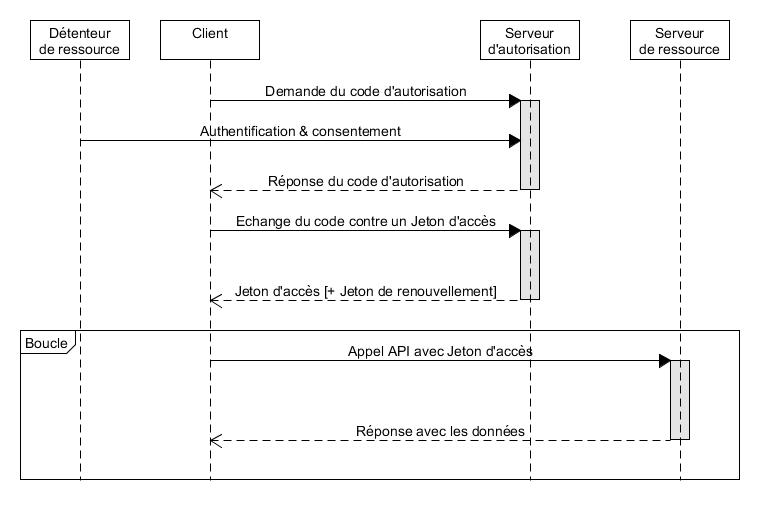
\includegraphics[width=0.85\textwidth]{img/authorization_code.jpg}
	\caption{Diagramme de s{\'e}quence -- L'autorisation via un code}
\end{figure} ~\\

\underline{Exemple :}
\begin{itemize}
	\item[$>$] D{\'e}tenteur des donn{\'e}es (Resource Owner) : vous
	\item[$>$] Serveur de ressources (Resource Server) : un serveur Facebook
	\item[$>$] Client (Client Application) : un site internet quelconque
	\item[$>$] Serveur d'autorisation (Authorization Server) : un serveur Facebook
\end{itemize} ~\\

\underline{Sc{\'e}nario :}
\begin{itemize}
	\item[$\bullet$] Le client souhaite acc{\'e}der aux informations de votre profil Facebook.
	\item[$\bullet$] Vous {\^e}tes redirig{\'e} par le client vers le serveur d'autorisation.
	\item[$\bullet$] Si vous autorisez l'acc{\`e}s, le serveur d'autorisation envoie un code d'autorisation au client.
	\item[$\bullet$] Ce code est {\'e}chang{\'e} par un token d'acc{\`e}s de fa\c{c}on transparente pour vous.
	\item[$\bullet$] Le client peut donc maintenant utiliser ce token d'acc{\`e}s pour acc{\'e}der aux donn{\'e}es de votre profil par le serveur de ressources.
\end{itemize}

\subsection*{L'autorisation implicite (Implicit Grant)\markboth{L'autorisation implicite (Implicit Grant)}{L'autorisation implicite (Implicit Grant)}}
\addcontentsline{toc}{subsection}{L'autorisation implicite (Implicit Grant)}

L'autorisation implicite est utilis{\'e}e pour obtenir seulement un jeton d'acc{\`e}s. Il ne permet pas d'obtenir le jeton de renouvellement. Il est optimis{\'e} pour un client de type public qui est g{\'e}n{\'e}ralement mis en \oe uvre dans un navigateur en utilisant un langage de script. ~\\

L'inconv{\'e}nient :
\begin{itemize}
	\item[$>$] Il expose le jeton d'acc{\`e}s c{\^o}t{\'e} client
\end{itemize}

\begin{figure}[ht]
	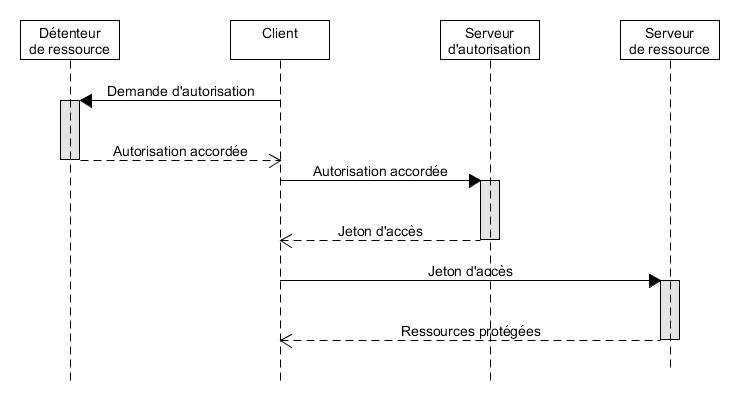
\includegraphics[width=0.85\textwidth]{img/implicit.jpg}
	\caption{Diagramme de s{\'e}quence -- L'autorisation implicite}
\end{figure}

\underline{Exemple :}
\begin{itemize}
	\item[$>$] D{\'e}tenteur des donn{\'e}es (Resource Owner) : vous
	\item[$>$] Serveur de ressources (Resource Server) : un serveur Facebook
	\item[$>$] Client (Client Application) : un site internet utilisant AngularJS par exemple
	\item[$>$] Serveur d'autorisation (Authorization Server) : un serveur Facebook
\end{itemize}

\underline{Sc{\'e}nario :}
\begin{itemize}
	\item[$\bullet$] Le client souhaite acc{\'e}der aux informations de votre profil Facebook.
	\item[$\bullet$] Vous {\^e}tes redirig{\'e} par le navigateur web vers le serveur d'autorisation.
	\item[$\bullet$] Si vous autorisez l'acc{\`e}s, le serveur d'autorisation vous redirige sur le client et met {\`a} disposition le token d'acc{\`e}s dans le fragment de l'url (non envoy{\'e} au serveur web). Exemple de callback : \texttt{http://example.com/oauthcallback\#access\_token=MzJmNDc3M2VjMmQzN}.
	\item[$\bullet$] Ce token d'acc{\`e}s peut maintenant {\^e}tre utilis{\'e} (apr{\`e}s avoir {\'e}t{\'e} valid{\'e}) pour faire des appels {\`a} l'API Facebook via Javascript (par exemple \texttt{https://graph.facebook.com/me?access\_token=MzJmNDc3M2VjMmQzN)}.
\end{itemize}

\subsection*{L'autorisation via mot de passe (Resource Owner Password Credentials Grant)\markboth{L'autorisation via mot de passe (Resource Owner Password Credentials Grant)}{L'autorisation via mot de passe (Resource Owner Password Credentials Grant)}}
\addcontentsline{toc}{subsection}{L'autorisation via mot de passe (Resource Owner Password Credentials Grant)}

L'autorisation via mot de passe est utilis{\'e}e dans le cas o{\`u} le propri{\'e}taire de la ressource a une relation de confiance avec le client. En effet, les informations d'identification du propri{\'e}taire de ressource sont envoy{\'e}es au client. --- Elle est utilis{\'e}e pour obtenir en m{\^e}me temps un jeton d'acc{\`e}s et un jeton de renouvellement en {\'e}change des informations d'identification aupr{\`e}s du serveur d'autorisation. ~\\

\begin{figure}[ht]
	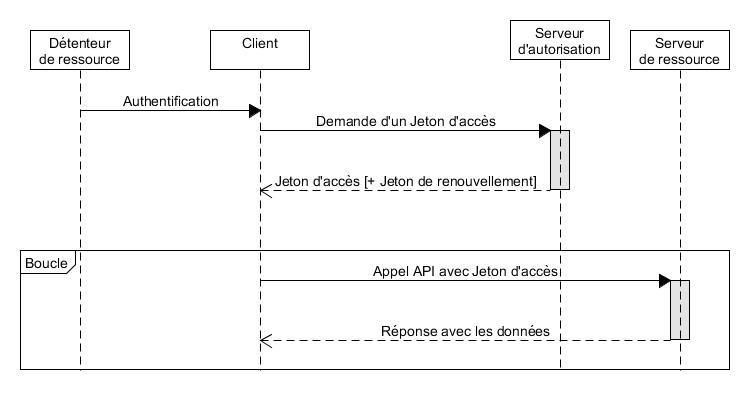
\includegraphics[width=0.85\textwidth]{img/Resource-Owner-Password-Credentials.jpg}
	\caption{Diagramme de s{\'e}quence -- L'autorisation via mot de passe}
\end{figure}

\underline{Exemple :}
\begin{itemize}
	\item[$>$] D{\'e}tenteur des donn{\'e}es (Resource Owner) : vous ayant un compte sur le site acme.com de la soci{\'e}t{\'e} Acme
	\item[$>$] Serveur de ressources (Resource Server) : la soci{\'e}t{\'e} Acme exposant son API {\`a} api.acme.com
	\item[$>$] Client (Client Application) : le site internet acme.com de la soci{\'e}t{\'e} Acme
	\item[$>$] Serveur d'autorisation (Authorization Server) : un serveur de la soci{\'e}t{\'e} Acme
\end{itemize}

\underline{Sc{\'e}nario :}
\begin{itemize}
	\item[$\bullet$] La soci{\'e}t{\'e} Acme fait les choses bien et a pens{\'e} {\`a} mettre {\`a} disposition {\`a} des applications tierces une API RESTful exposant tout plein de m{\'e}thodes pratiques pour r{\'e}cup{\'e}rer des donn{\'e}es diverses et vari{\'e}es de ses utilisateurs.
	\item[$\bullet$] Cette soci{\'e}t{\'e} se dit qu'il serait pratique d'utiliser sa propre API pour {\'e}viter de r{\'e}inventer la roue et de maintenir du code {\`a} plusieurs endroits.
	\item[$\bullet$] Elle a donc besoin d'un token d'acc{\`e}s pour appeler les m{\'e}thodes de son API.
	\item[$\bullet$] Pour cela elle vous demande de renseigner vos identifiants de connexion via un formulaire HTML classique tel que vous le faites habituellement.
	\item[$\bullet$] L'application c{\^o}t{\'e} serveur (le site acme.com) va {\'e}changer vos identifiants contre un token d'acc{\`e}s aupr{\`e}s du serveur d'autorisation (si vos identifiants sont valides bien {\'e}videmment).
	\item[$\bullet$] L'application peut donc maintenant utiliser ce token d'acc{\`e}s aupr{\`e}s du serveur de ressources (api.acme.com).
\end{itemize}

\subsection*{L'autorisation serveur {\`a} serveur (Client Credentials Grant)\markboth{L'autorisation serveur {\`a} serveur (Client Credentials Grant)}{L'autorisation serveur {\`a} serveur (Client Credentials Grant)}}
\addcontentsline{toc}{subsection}{L'autorisation serveur {\`a} serveur (Client Credentials Grant)}

L'autorisation serveur {\`a} serveur est utilis{\'e}e dans le cas o{\`u} le client est lui-m{\^e}me d{\'e}tenteur de donn{\'e}es. Il n'y a pas d'autorisation {\`a} obtenir de la part de l'utilisateur final. ~\\

Le client peut demander un jeton d'acc{\`e}s en utilisant uniquement ses informations d'identification client lorsqu'il a demand{\'e} l'acc{\`e}s {\`a} des ressources prot{\'e}g{\'e}es sous son contr{\^o}le.

\begin{figure}[ht]
	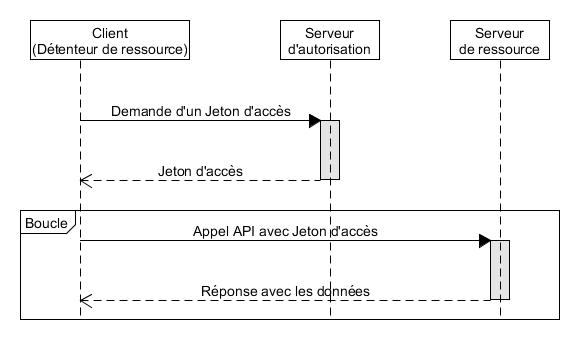
\includegraphics[width=0.85\textwidth]{img/client_credentials.jpg}
	\caption{Diagramme de s{\'e}quence -- L'autorisation serveur {\`a} serveur}
\end{figure}

\underline{Exemple :}
\begin{itemize}
	\item[$>$] D{\'e}tenteur des donn{\'e}es (Resource Owner) : un site internet quelconque
	\item[$>$] Serveur de ressources (Resource Server) : Google Cloud Storage
	\item[$>$] Client (Client Application) : le d{\'e}tenteur des donn{\'e}es
	\item[$>$] Serveur d'autorisation (Authorization Server) : un serveur Google
\end{itemize}

\underline{Sc{\'e}nario :}
\begin{itemize}
	\item[$\bullet$] Un site internet quelconque stocke des fichiers de toute sorte sur Google Cloud Storage.
	\item[$\bullet$] Le site internet doit passer par l'API Google pour r{\'e}cup{\'e}rer ou modifier des fichiers et doit donc s'authentifier aupr{\`e}s du serveur d'autorisation.
	\item[$\bullet$] Une fois authentifi{\'e}, le site internet obtient un token d'acc{\`e}s qu'il peut d{\'e}sormais utiliser aupr{\`e}s du serveur de ressources .
\end{itemize}

\section*{Conclusion\markboth{Conclusion}{Conclusion}}
\addcontentsline{toc}{section}{Conclusion}

Nous avons vu les notions de base du protocole OAuth 2.0 . OAuth 2.0 est devenu un standard pour la d{\'e}l{\'e}gation d'autorisation entre diff{\'e}rentes applications. Les grands firmes l'ont adopt{\'e} et pourquoi pas vous ? ~\\
Enfin une derni{\`e}re chose, si vous souhaitez utiliser ce protocole dans vos applications, il faut veiller scrupuleusement {\`a} la s{\'e}curit{\'e}. Le protocole propose des solutions plus ou moins facile {\`a} mettre en œuvre. ~\\

\subsection*{Ressources Web\markboth{Ressources Web}{Ressources Web}}
\addcontentsline{toc}{subsection}{Ressources Web}

OAuth 2.0 : \texttt{http://oauth.net/2/} , \texttt{http://tools.ietf.org/html/rfc6749}~\\
S{\'e}curit{\'e}s OAuth 2.0 : \texttt{http://tools.ietf.org/html/rfc6819}

%% \subsection*{MatrixQueryLanguage\markboth{MatrixQueryLanguage}{MatrixQueryLanguage}}
%% \addcontentsline{toc}{subsection}{MatrixQueryLanguage}

\clearpage

%% \section*{Bibliographie\markboth{Bibliographie}{Bibliographie}}
%% \addcontentsline{toc}{section}{Bibliographie}
%% \nocite{*}
%% %toutes references biblio : 6 lettres + 2 chiffres
%% \bibliography{document}
%% \bibliographystyle{frplain} % plain or frplain

\end{document}
